\chapter{Channel Modeling}
As the controller is run on two different servers, a link between these have to be established and modeled. The connection is seen as a connection from a server (ex. a "mothership") and a client (ex. AAUSHIP). Where the communication goes both ways, as the server needs to compute what the client should do next based on measurements from the client, and the client needs to respond to these data. Figure \vref{fig:chanmod} is an illustration of the communication. 

\begin{figure}[htbp]
		\begin{center}
			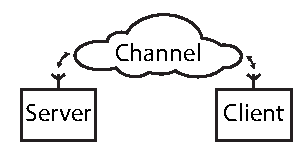
\includegraphics[width=8.4cm]{img/chanmod}
			\caption{Depiction of the communication link between the server and the client.}
			\label{fig:chanmod}
		\end{center}
\end{figure}

As the protocol between the server and the client, includes a validity check, the channel estimation becomes a simple question of wether or not the received package is valid or not - thus it can be estimated using a bernoulli distribution of the packages. The channel $\gamma$ is modeled using the bernoulli distribution which has a probability mass function that can be described as:
\begin{align}
\gamma[n] = 
\left\{ 
  \begin{array}{l l}
    p & \quad \text{for}\,\, \gamma[n] = 1\\
    q & \quad \text{for}\,\, \gamma[n] = 0
  \end{array} \right.
\end{align}
For $n = 0,1,2,\dots$ and $q = (1-p)$. To determine the probability of succes $p$, a test have been carried out, where the device was held steady at a distance, to determine the PMF of the packet losses - which are used to estimate wether a packet is received or not. This test has been used to determine these factors, and the worst case scenario have been used, as the actual probability will always be better than this. 



Test results show that the communication link at a distance of X metres begin to have quite a high loss ratio with the current equipment mounted on the ship - and so the ship should never be further away, as communication begins to become faulty. To verify if the ship can still navigate without sending packets back and forth 

As the server and client are independent devices the joint probability is equal to the product of their functions, 